
C++11引入了右值引用来支持新的特性,包括移动语义和完善转发。本节描述右值引用和类型推导之间的交互。

\subsubsubsection{15.6.1\hspace{0.2cm}引用折叠规则}

开发者不允许直接声明“引用的引用”:

\begin{lstlisting}[style=styleCXX]
using RI = int&;
int i = 42;
RI r = i;
R const& rr = r; // OK: rr has type int&
\end{lstlisting}

确定由这样的组合产生的类型的规则称为引用折叠规则。

\begin{tcolorbox}[colback=webgreen!5!white,colframe=webgreen!75!black]
\hspace*{0.75cm}当人们注意到标准pair类模板不能使用引用类型时,引用折叠就引入了C++2003标准中。2011年的标准进一步扩展了右值引用的规则。
\end{tcolorbox}

首先,应用于内部引用之上的const或volatile限定符都会丢弃(只有内部引用之下的限定符会保留)。根据表15.1,这两个引用会简化为一个引用,可以总结为“如果其中一个引用是左值引用,得到的类型也是左值引用;否则,就是一个右值引用。”

\begin{center}
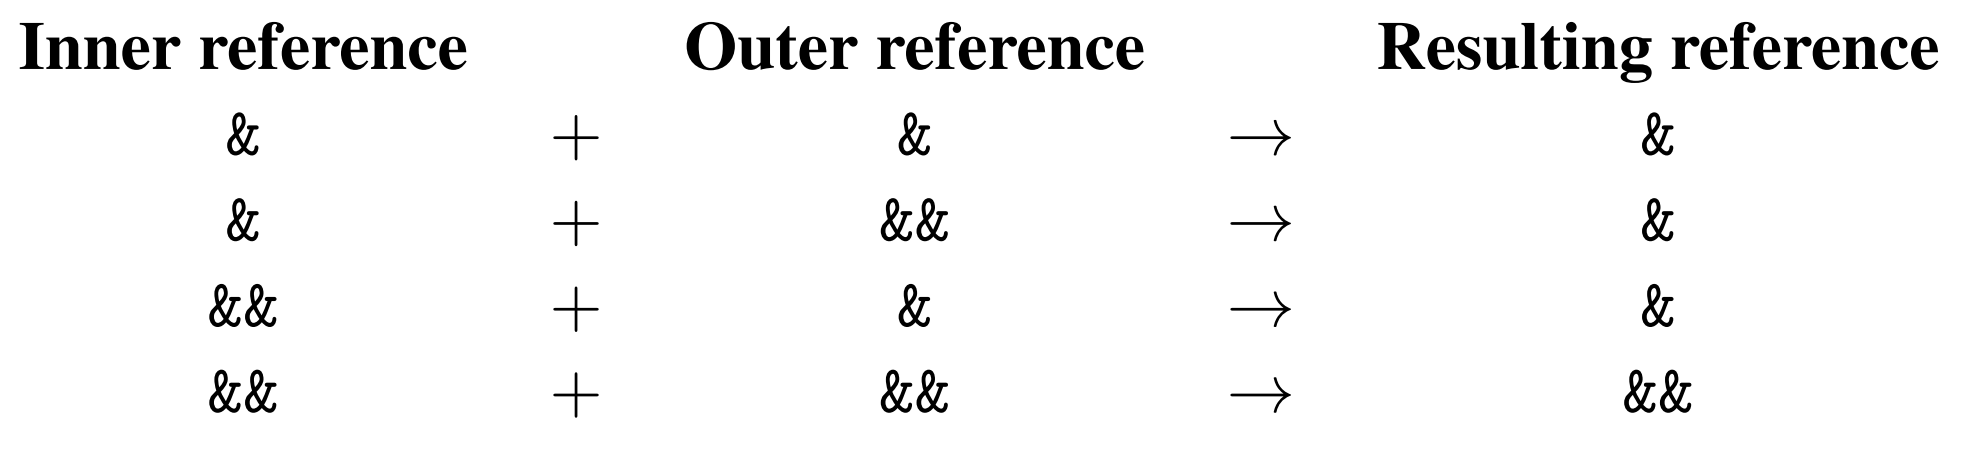
\includegraphics[width=0.8\textwidth]{content/2/chapter15/images/1.png} \\
表15.1. 引用折叠规则
\end{center}

还有一个例子展示了这些规则的实际应用:

\begin{lstlisting}[style=styleCXX]
using RCI = int const&;
RCI volatile&& r = 42; // OK: r has type int const&
using RRI = int&&;
RRI const&& rr = 42; // OK: rr has type int&&
\end{lstlisting}

volatile应用于引用类型RCI(int const\&的别名),因此丢弃。然后,右值引用位于该类型的顶部,但是由于基础类型是左值引用,并且左值引用在引用折叠规则中“优先”,所以整体类型保持int const\&(或RCI,是一个等效别名)。类似地,丢弃RRI上的const,并且在产生的右值引用类型上应用右值引用,最后留下一个右值引用类型(能像42那样绑定右值)。

\subsubsubsection{15.6.2\hspace{0.2cm}转发引用}

在6.1节中介绍的,当函数参数是转发引用(对该函数模板参数的右值引用)时,模板参数推导会以一种特殊的方式进行。在这种情况下,模板参数推导不仅要考虑函数调用参数的类型,还要考虑该参数是左值还是右值。在参数是左值的情况下,由模板参数推导确定的类型为参数类型的左值引用,引用折叠规则(见上面)确保替换的参数是左值引用。否则,为模板参数推导出的类型就是参数类型(不是引用类型),而替换的参数是该类型的右值引用。例如:

\begin{lstlisting}[style=styleCXX]
template<typename T> void f(T&& p); // p is a forwarding reference

void g()
{
	int i;
	int const j = 0;
	f(i); // argument is an lvalue; deduces T to int& and
	// parameter p has type int&
	f(j); // argument is an lvalue; deduces T to int const&
	// parameter p has type int const&
	f(2); // argument is an rvalue; deduces T to int
	// parameter p has type int&&
}
\end{lstlisting}

在调用f(i)时,模板参数T推导为int\&,因为表达式i是int类型的左值。将int\&替换为T的参数类型T\&\&需要引用折叠,这里使用\& + \&\& \texttt{->} \&的规则,得到的参数类型是int\&,适合接受int类型的左值。相反,f(2)中参数2是一个右值,因此模板参数推导为该右值的类型(即int)。生成的函数参数不需要引用折叠,类型为int\&\&(同样,适合的参数)。

将T推导为引用类型会对模板的实例化产生一些有趣的影响。例如,用T类型声明的局部变量在左值实例化后具有引用类型,因此需要初始化式:

\begin{lstlisting}[style=styleCXX]
template<typename T> void f(T&&) // p is a forwarding reference
{
	T x; // for passed lvalues, x is a reference
	...
}
\end{lstlisting}

上面函数f()的定义需要注意如何使用T类型,否则函数模板本身在使用左值参数时将无法正常工作。为了处理这种情况,常使用std::remove\_reference类型特性来确定x不是一个引用:

\begin{lstlisting}[style=styleCXX]
template<typename T> void f(T&&) // p is a forwarding reference
{
	std::remove_reference_t<T> x; // x is never a reference
	...
}
\end{lstlisting}


\subsubsubsection{15.6.3\hspace{0.2cm}完美转发}

右值引用的特殊推导规则和引用折叠规则的结合,使编写一个函数模板成为可能,其参数可以接受任何参数,并捕获其属性(类型,以及它是左值还是右值)。

\begin{tcolorbox}[colback=webgreen!5!white,colframe=webgreen!75!black]
\hspace*{0.75cm}位字段是个例外。
\end{tcolorbox}

然后,函数模板可以将参数“转发”到另一个函数,如下所示:

\begin{lstlisting}[style=styleCXX]
class C {
	...
};

void g(C&);
void g(C const&);
void g(C&&);

template<typename T>
void forwardToG(T&& x)
{
	g(static_cast<T&&>(x)); // forward x to g()
}

void foo()
{
	C v;
	C const c;
	forwardToG(v); // eventually calls g(C&)
	forwardToG(c); // eventually calls g(C const&)
	forwardToG(C()); // eventually calls g(C&&)
	forwardToG(std::move(v)); // eventually calls g(C&&)
}
\end{lstlisting}

上面演示的技术称为完美转发,通过forwardToG()间接调用g()的结果将与直接调用g()的代码相同:不生成副本。

forwardToG()函数中使用static\_cast需要一些解释。在forwardToG()的实例化中,参数x要么具有左值引用类型,要么具有右值引用类型。无论如何,表达式x将是引用所引用类型的左值。

\begin{tcolorbox}[colback=webgreen!5!white,colframe=webgreen!75!black]
\hspace*{0.75cm}将右值引用类型的参数作为左值处理是出于安全考虑,因为带有名称的参数可以很容易地在函数中多次引用。如果这些引用中的每一个都可以隐式地作为右值,那么其值就可以在开发者不知道的情况下销毁。因此,必须显式声明命名实体何时视为右值。为此,C++标准库函数std::move将其操作的值视为右值(或者更准确地说,xvalue;详见附录B)。
\end{tcolorbox}

static\_cast将x转换为原始类型和左值或右值。类型T\&\&要么折叠为左值引用(如果原始参数是左值,则T是左值引用),要么会是右值引用(如果原始参数是右值),因此static\_cast的结果具有与原始参数相同的类型和左值或右值性,从而实现完美转发。

正如在第6.1节中介绍的,C++标准库在头文件<utility>中提供了一个函数模板std::forward<>(),该函数模板应用于替代static\_cast以实现完美转发。使用该程序模板比上面的不透明static\_cast更好地记录了开发者的意图,并防止了遗漏\&等错误。也就是说,上面的例子可以写得更清楚:

\begin{lstlisting}[style=styleCXX]
#include <utility>

template<typename T> void forwardToG(T&& x)
{
	g(std::forward<T>(x)); // forward x to g()
}
\end{lstlisting}

\hspace*{\fill} \\ %插入空行
\noindent
\textbf{完美转发可变参数模板}

完美转发与可变参数模板可以很好的结合,允许函数模板接受任意数量的函数调用参数,并将每个参数转发给另一个函数:

\begin{lstlisting}[style=styleCXX]
template<typename... Ts> void forwardToG(Ts&&... xs)
{
	g(std::forward<Ts>(xs)...); // forward all xs to g()
}
\end{lstlisting}

forwardToG()调用中的参数将(独立地)推导参数包Ts的连续值(参见第15.5节),以便捕获每个参数的类型和左值或右值。调用g()中的包扩展(参见第12.4.1节)将使用上面解释的完美转发,转发每个参数。

尽管称为完美转发,但并不是“完美”的,因为没有捕捉到一个表达式的所有属性。例如,不区分左值是否是位域左值,也不捕获表达式是否具有特定的常量值。后者会引起问题,特别是处理空指针常量时,这是一个整型值,计算结果为常量0。由于完美转发无法捕获表达式的常量值,因此在下面的例子中,对g()的直接调用与对g()的转发调用会有不同的行为:

\begin{lstlisting}[style=styleCXX]
void g(int*);
void g(...);

template<typename T> void forwardToG(T&& x)
{
	g(std::forward<T>(x)); // forward x to g()
}

void foo()
{
	g(0); // calls g(int*)
	forwardToG(0); // eventually calls g(...)
}
\end{lstlisting}

这也是使用nullptr(C++11中引入),而不是空指针常量的另一个原因:

\begin{lstlisting}[style=styleCXX]
g(nullptr); // calls g(int*)
forwardToG(nullptr); // eventually calls g(int*)
\end{lstlisting}

所有的完美转发示例都专注于转发函数参数,同时保持它们类型,以及是左值还是右值。当将调用的返回值转发给另一个函数时,也会出现同样的问题,该函数的类型和值类型完全相同,即在附录B中讨论的左值和右值。C++11中引入的decltype功能(在第15.10.2节)允许使用这种有点冗长的惯用法:

\begin{lstlisting}[style=styleCXX]
template<typename... Ts>
auto forwardToG(Ts&&... xs) -> decltype(g(std::forward<Ts>(xs)...))
{
	return g(std::forward<Ts>(xs)...); // forward all xs to g()
}
\end{lstlisting}

注意,return语句中的表达式会逐字复制到decltype类型中,以便计算返回表达式的确切类型。此外,还使用了末尾的返回类型特征(即,函数名之前的自动占位符和\texttt{->}来指示返回类型),以便函数参数包xs在decltype类型的范围内。这个转发函数“完美”地将所有参数转发给g(),然后“完美”地将其结果转发回调用者。

C++14引入了其他特性进一步简化这种情况:

\begin{lstlisting}[style=styleCXX]
template<typename... Ts>
decltype(auto) forwardToG(Ts&&... xs)
{
	return g(std::forward<Ts>(xs)...); // forward all xs to g()
}
\end{lstlisting}

使用decltype(auto)作为返回类型表明编译器应该从函数的定义,推导出返回类型。参见15.10.1节和15.10.3节。

\subsubsubsection{15.6.4\hspace{0.2cm}惊奇推导}

对右值引用的特殊推导规则结果,对完善转发具有重要意义。然而,也可能会令人惊讶,因为函数模板通常在函数签名中泛化类型,而不影响参数类型(左值或右值)。考虑一下这个例子:

\begin{lstlisting}[style=styleCXX]
void int_lvalues(int&); // accepts lvalues of type int
template<typename T> void lvalues(T&); // accepts lvalues of any type

void int_rvalues(int&&); // accepts rvalues of type int
template<typename T> void anything(T&&); // SURPRISE: accepts lvalues and
// rvalues of any type
\end{lstlisting}

将具体函数(如int\_rvalues)抽象到模板等价物的开发者,可能会对函数模板接受左值感到惊讶。幸运的是,这种推导行为仅适用于以下情况:函数参数是用表单模板参数\&\&编写的,是函数模板的一部分,并且命名的模板参数由该函数模板声明。因此,该推导规则不适用于以下情况:

\begin{lstlisting}[style=styleCXX]
template<typename T>
class X
{
	public:
	X(X&&); // X is not a template parameter
	X(T&&); // this constructor is not a function template
	
	template<typename Other> X(X<U>&&); // X<U> is not a template parameter
	template<typename U> X(U, T&&); // T is a template parameter from
	// an outer template
};
\end{lstlisting}

尽管这个模板推导规则给出了令人惊讶的行为,但在实践中,这种行为导致问题的情况并不常见。当它发生时,可以使用SFINAE(参见第8.4节和第15.7节)和类型特征,如std::enable\_if(参见第6.3节和第20.3节)来限制模板只能接收右值:

\begin{lstlisting}[style=styleCXX]
template<typename T>
typename std::enable_if<!std::is_lvalue_reference<T>::value>::type
rvalues(T&&); // accepts rvalues of any type
\end{lstlisting}


























